\section{Umsetzung}
Hier werden konkret alle Aspekte der Umsetzung der in \cref{specification} bereits beschriebenen Spezifikation behandelt. %TODO umschreiben
 
\subsection{Initiales Aufsetzen der Anwendung}
Bevor die Entwicklung starten kann müssen die grundlegende Bausteine der Anwendung angelegt, konfiguriert und verbunden werden. 

\subsubsection{Spring Boot Anwendung}
Spring stellt eine Weboberfläche zur Verfügung, in der ein komplettes Spring Boot Projekt inklusive Abhängigkeiten einfach generiert werden kann. Die Oberfläche (nachstehend Spring Initializr) erlaubt es Maven oder Gradle als Build-Management-Tool zu verwenden. In diesem Projekt fiel die Entscheidung für Maven, aufgrund der bereits vorhandenen Erfahrung mit dem Tool. 

\begin{figure}[th!]
	\centering
	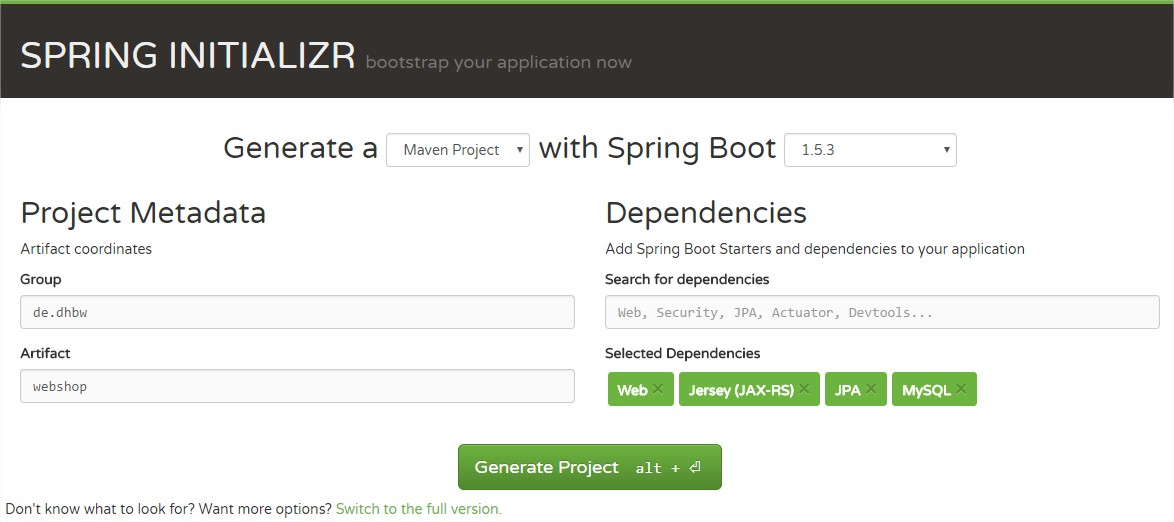
\includegraphics[width=\linewidth]{bilder/kap7/Spring-Initializr}
	\caption{Spring Inititalizr Weboberfläche\cite{}}
	\label{fig:spring-initializr}
\end{figure}

\cref{fig:spring-initializr} zeigt die gewählte Konfiguration für das Grundprojekt. Links sind die Metadaten für das Deployment definiert und rechts die Abhängigkeiten. Diese sind initial:
\begin{itemize}
	\item Web. Benötigt um eine Webanwendung mit eingebetteten Tomcat-Server zu implementieren.
	\item Jersey. 
\end{itemize}


\subsubsection{Angular 2 Anwendung}
angular2 scaffolding mit angular cli (erklären was es ist) und initiale Konfiguration bzw Anbindung mit spring boot app

\subsection{Datenbank}


\subsection{Backend-Klassen und ORM}
Eine Klasse pro Entität in der Datenbank + DAO-Klasse, Beispiele für die Realisierung von Beziehungen usw. zeigen (ORM-Annotationen)

\subsection{Webservices}
Jersey erklären (was es ist, Konfiguration), Aufbau der Rest-Interfaces + Implementierungen, evtl. Klassendiagramme. 

\subsection{Frontend}
Erstellte Module in Angular 2 (was sind Module? -> Erklären), Struktur von Komponenten, Hauptkomponenten der Module, Services, Routing